\documentclass[thesis]{subfiles}

\begin{document}

\chapter{Adsorption and intrusion in nanoporous materials}

\section{Porous materials}

Porous materials are material presenting a structural porosity, their
tri-dimensional structure showing cavities called \emph{pores}. This pores
network can vary in homogeneity and regularity, creating a wide variety of
porous materials. They all have in common a high specific surface area, which is
the accessible internal surface by grams of the material --- up to thousands of
square meters by gram of material\cite{Farha2012} in the most extreme cases.
This very high specific surface area of porous materials is exploited in a
number of important industrial applications, especially in the domains of
adsorption and catalysis. For example, porous materials are used to separate
gases in mixtures as molecular sieves; to filter and remove heavy metals from
water; or in heterogeneous catalysis in oil refineries by the cracking process.

The International Union for Pure and Applied Chemistry (IUPAC) recommends to
classify porous materials in three groups, depending on the size of the
pores\cite{Rouquerol1994}. First are the \emph{microporous} solids, where the
pores are less than \SI{2}{nm} in diameter. Then we find the \emph{mesoporous}
solids with pore diameter between 2 and \SI{50}{nm}. Porous solids with pores
larger than \SI{50}{nm} are called \emph{macroporous} solids. Microporous and
mesoporous solids are often grouped together as \emph{nanoporous} solids, where
the size of pores does not exceed \SI{50}{nm}.

\begin{figure}[ht]
    \centering
    \raisebox{-0.5\height}{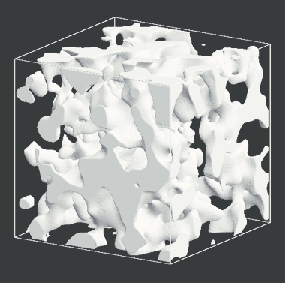
\includegraphics[width=0.3\textwidth]{figures/cited/porous-vycor}}
    \hfill
    \raisebox{-0.5\height}{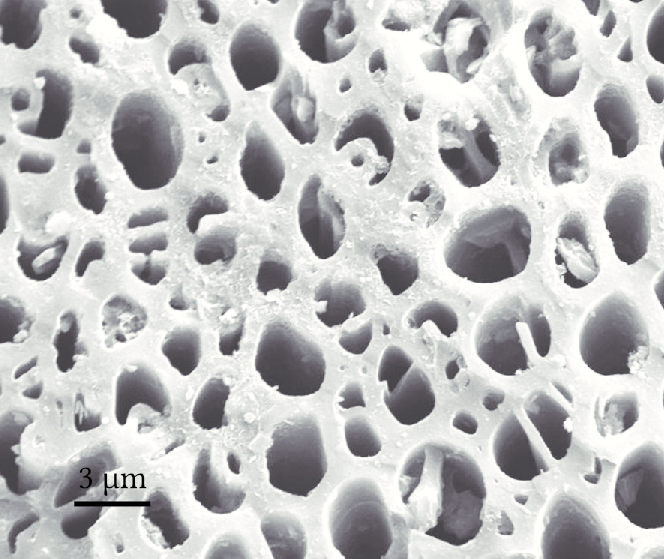
\includegraphics[width=0.3\textwidth]{figures/cited/porous-carbon}}
    \hfill
    \raisebox{-0.5\height}{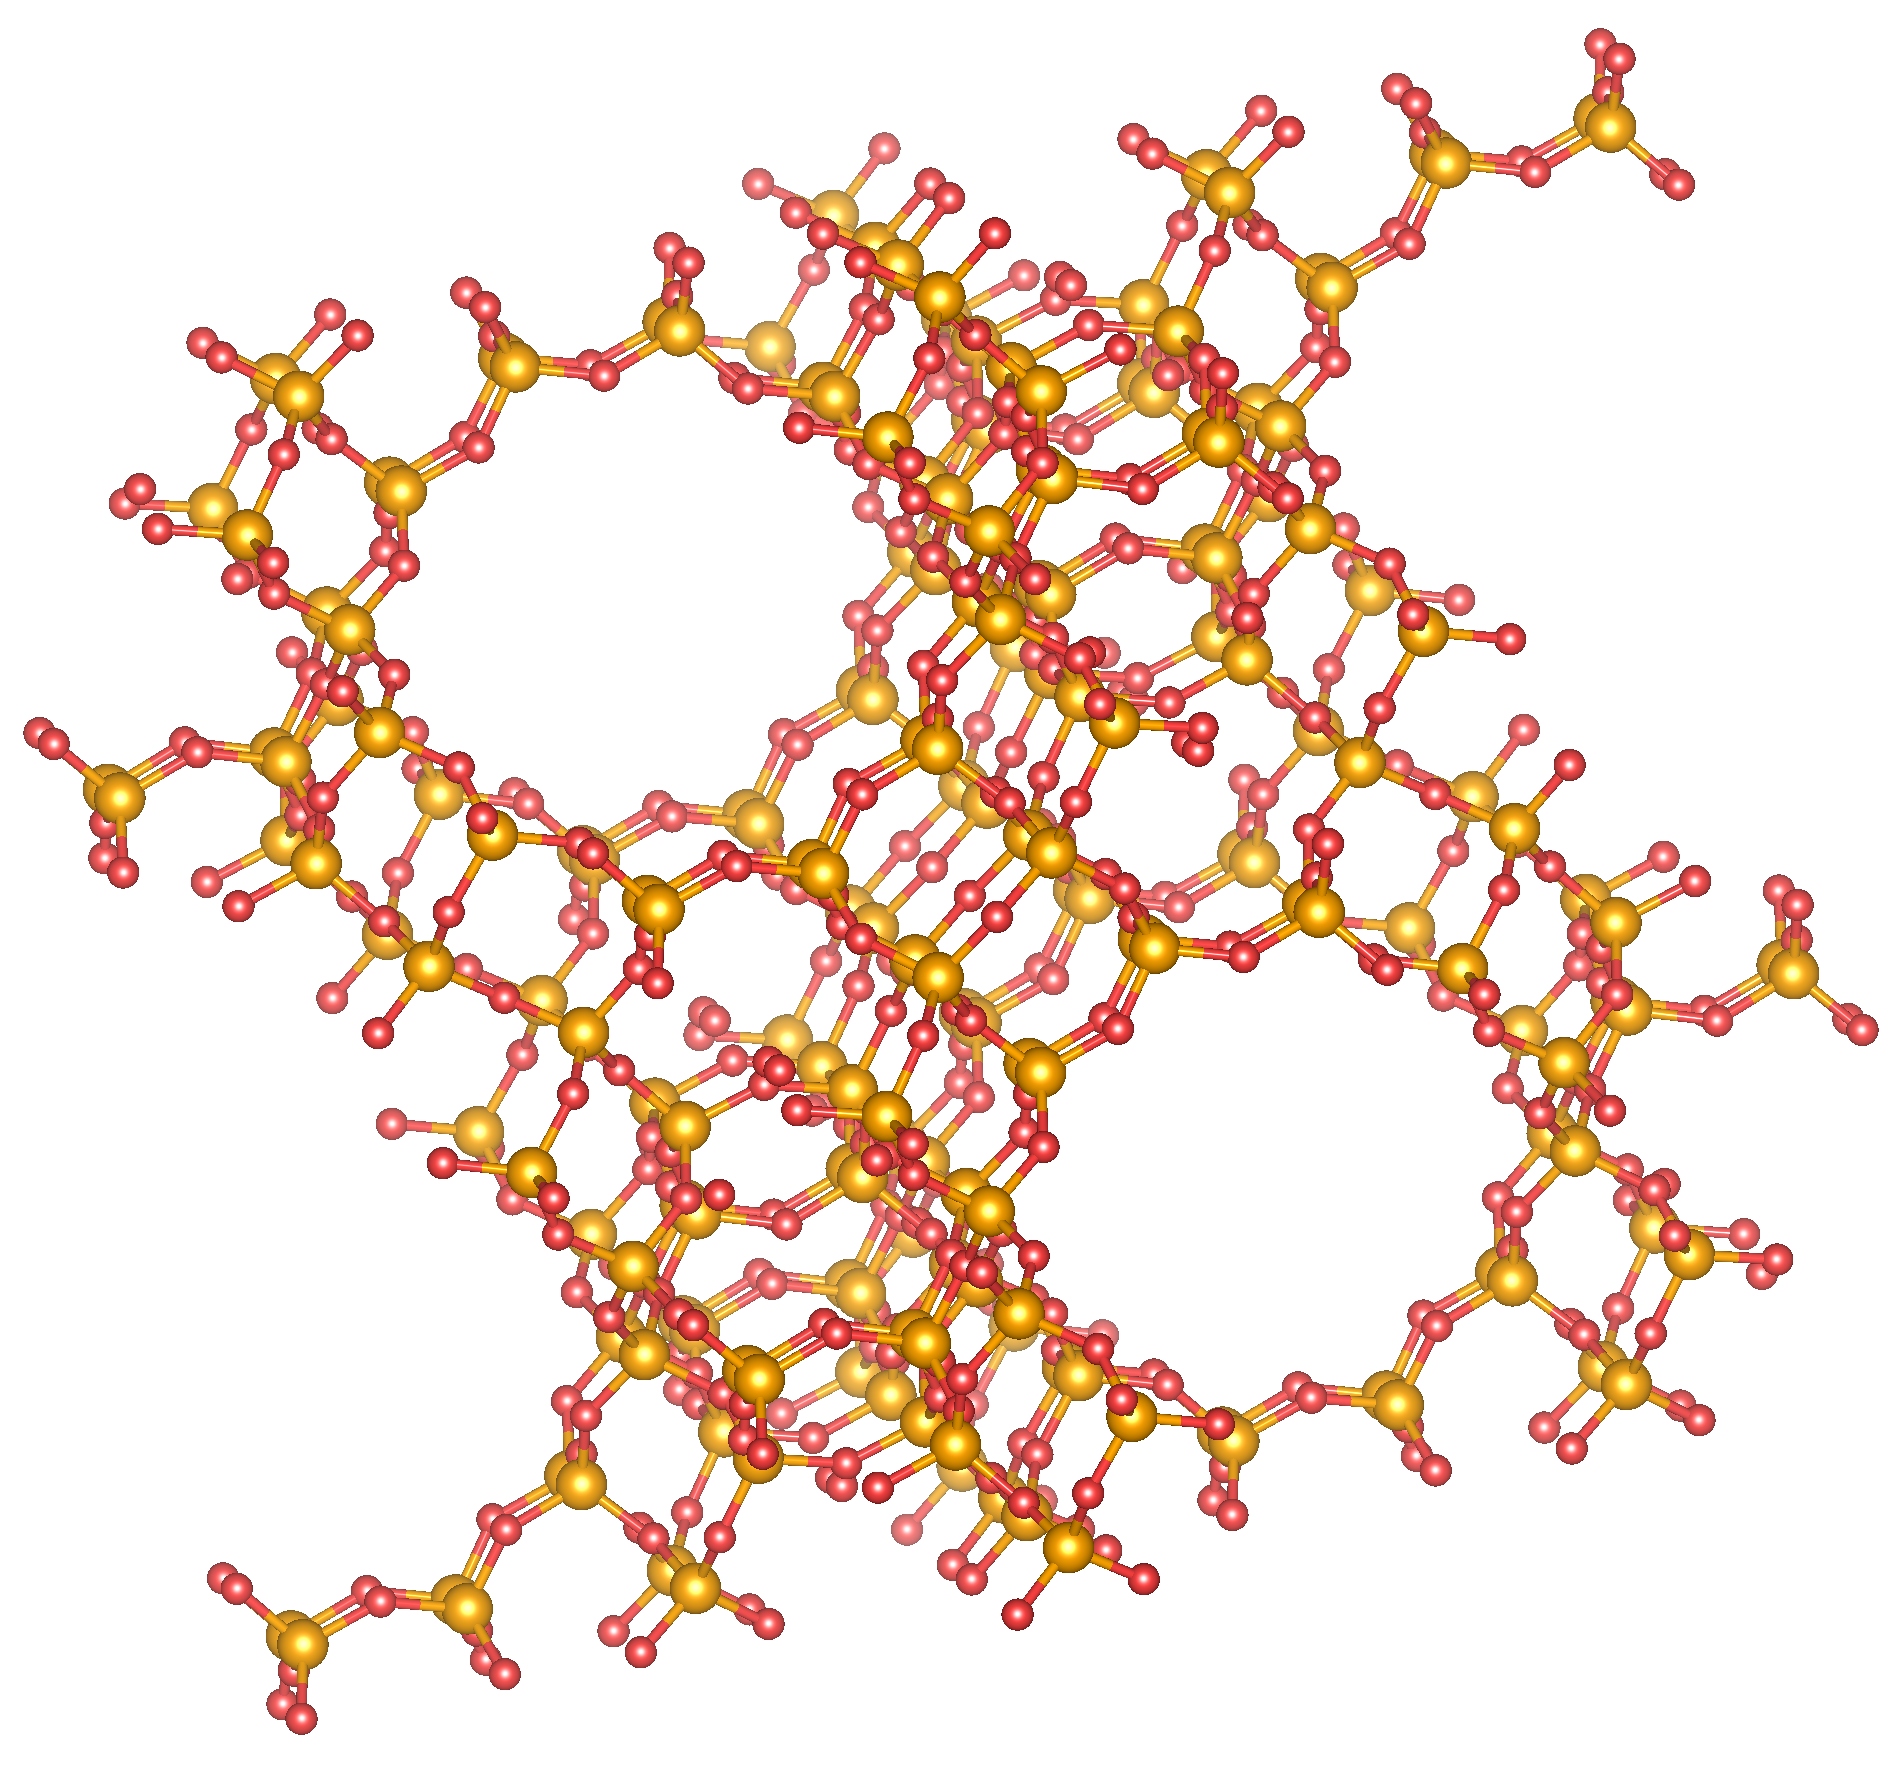
\includegraphics[width=0.3\textwidth]{figures/cited/porous-faujasite}}
    \caption{Three examples of porous material. The left image is a
    representation of a vycor glass (disordered)\cite{Levitz2003}; the middle
    is a scanning electron microscope image of activated carbon (ordered but non
    crystalline)\cite{Das2015}; and right is the crystalline structure of the
    zeolite faujasite.}
    \label{fig:porous-examples}
\end{figure}

Porous materials are also classified depending on their structural regularity,
from highly regular crystalline materials such as zeolites and
\emph{Metal-Organic Frameworks} (MOFs) showing a periodic organization of their
atoms; to regular porous materials such as clays and carbon nanotubes, where the
porosity is well defined but does not present long-distance ordering. Finally,
there also exist amorphous porous materials, which have a wide distribution of
pore sizes and shapes, an no periodicity. Examples in this latter class are
vycor glasses, silica glasses, or aerogels. Three example of porous solids with
different pore size and regularity are presented in
figure~\ref{fig:porous-examples}.

A final distinction we can make among porous materials is the one of their
chemical nature. They are usually classified as either organic or inorganic
materials. The former contains materials build around carbon atoms, such as
carbon nanotubes, or porous polymers. The latter class have historically been
the widest one, containing materials such as oxides, alumino-silicates, sulfurs
compound or alumino-phosphates. In the last few decades, we have seen blooming a
new class of materials, with an hybrid inorganic-organic composition. This new
family contains organo-silicic material, and \emph{Metal-Organic Frameworks}
which have been the main subject of study in my PhD.

During my PhD, I studied hybrid inorganic-organic crystalline nanoporous
materials, and especially flexible ones. In the next sections, I will describe
zeolites as the conventional example of crystalline porous material, and MOFs as
the relatively new class of hybrid inorganic-organic porous materials. I will
also present the \emph{Zeolitic Imidazolate Framework} (ZIF) family of MOFs,
which are MOFs with a zeolite topology.

\subsection{Zeolites}

% Zeolites where named by the Swedish mineralogist Axel Fredrik Crönsted in
% 1756\cite{Ferey2001} from the Greek \textgreek{ζέω} (zéō), meaning "to boil"
% and \textgreek{λίθος} (líthos), meaning "stone".
He observed that when heating a fragment of stibilite mineral to 150°C, the
stone started to cover itself with small bubbles, coming from water adsorbed
inside, as if the stone was starting to boil. In the following decades, around
twenty additional natural zeolites have been discovered. In 1862, French chemist
Henri Sainte-Claire Deville, created the first artificial analog to zeolites,
but it was only in 1930, that Linus Pauling resolved the structure of zeolites
using X rays diffraction. Today, 234 unique zeolite frameworks have been
identified, and we know over 65 naturally occurring zeolite frameworks according
to the International Zeolite Association\cite{iza-website}.

\subsubsection{Structure and composition}

Zeolites are porous crystalline alumino-silicate, with a structure built around
a regular arrangement of \ce{SiO4} or \ce{AlO4} tetrahedra linked together by
their vertices as represented in figure~\ref{fig:zeolite-building-block}. The
porous network created by these tetrahedra is very different from one zeolite to
another, resulting in a wide variety of materials and properties. For examples,
the pores can be linear, spherical or in a zig-zag disposition; connected
together through windows or independents. The International Zeolite Association
gives a three letter code such as LTA, FAU or SOD to each experimental
crystalline structure. It is however mathematically possible to generate an
infinite number of crystalline structures using tetrahedra as a building block;
and there are databases of hypothetical zeolites with more than 2 million
different frameworks\cite{hypothetical-zeolites}.

\begin{figure}[ht]
    \centering
    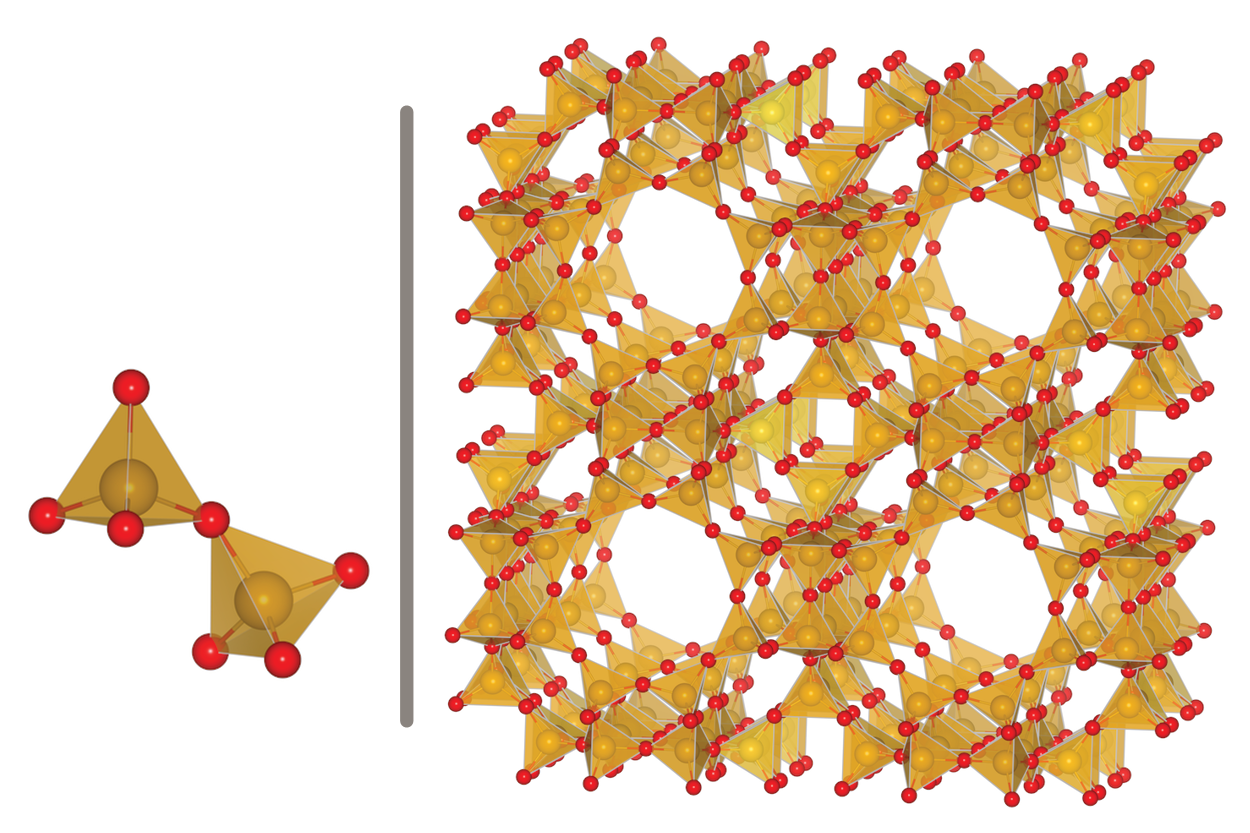
\includegraphics[width=0.75\textwidth]{figures/cited/zeolite-building-blocks}
    \caption{Two \ce{SiO4} tetrahedra on the right, and the structure of zeolite
    LTA on the left. Si atoms are in yellow and oxygen atoms in red.}
    \label{fig:zeolite-building-block}
\end{figure}

While silicate tetrahedra \ce{SiO4} are neutral, aluminum oxide tetrahedra
\ce{AlO4-} in the structure carry a negative charge, which is compensated in the
material by a counter ion such as sodium \ce{Na+}, potassium \ce{K+}, calcium
\ce{Ca^{2+}} or barium \ce{Ba^{2+}}. Because of this, each topology defines a
family of zeolite with varying chemical composition. The general chemical
formula for a zeolite is $\text{M}_{x/m}\, \text{Al}_x\, \text{Si}_{\,1-x}\,
\text{O}_2$. The Si/Al ratio can vary from 1 to infinity for purely silicic
zeolites, also called \emph{zeosil}. Each new aluminum atom replacing a silicon
atom is accompanied by a cation to ensure the overall charge neutrality. The
presence of these cations contributes to the remarkable adsorption and catalysis
properties of zeolites. They are used in industrial processes for ions exchange
through their extra cations; catalysis through their high specific surface area
and acido-basic properties; molecular sieves through the multiples pores sizes
and tuneable properties.

\newpage
\subsection{Metal--Organic Frameworks}

Metal--organic frameworks are a more recent class of crystalline nanoporous
materials. The first works on these materials were made in the 90 by Richard
Robson and collaborators\cite{Abrahams1991, Robson2008}, but the systematic
study of these materials only started in the 2000s. In 1999, the group of Omar
Yaghi created MOF-5\cite{Li1999}, a MOF with huge pores size (\SI{15}{\AA} in
diameter for the largest cavity), sparkling interest in the international
research community for these materials. Since then, the field of MOF has been
developing exponentially, both in terms of the number of publications and in
terms of number of structures reported in the literature.
Figures~\ref{fig:number-of-mofs} shows the growth of the number of structures in
the Cambridge Structural Database, with a doubling time of 3.9 years for
three-dimensional MOFs.

\begin{figure}[ht]
    \centering
    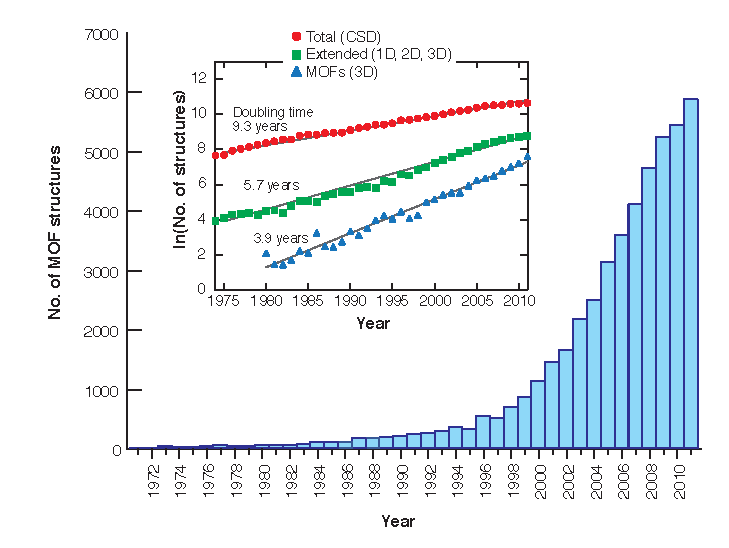
\includegraphics[width=0.7\textwidth]{figures/cited/number-of-mofs}
    \caption{Number of MOF structures in the Cambridge Structural Database
    showing an exponential growth. Image taken from reference~\cite{Furukawa2013}}
    \label{fig:number-of-mofs}
\end{figure}

Materials in the MOF family are built around metallic centers, connected by
organic linkers, assembled into nano- or mesoporous crystalline structures (see
figure~\ref{fig:mof-different-linkers}). Compared to zeolites, they can be
synthesized in a solvent at lower temperatures (from ambient temperature to
200°C), by mixing metallic salts and organic linkers. Because of these organic
linkers, MOFs have a smaller thermal stability (up to 400°C) compared to the
inorganic zeolites that can withstand up to 1000°C. Nevertheless, this reduced
stability is made up for by the incredible adaptability of the MOFs. By
combining linker-metal coordination chemistry variety with organic chemistry
adaptability, they offer a huge number of different structures, and can be tuned
for a specific application through linker and/or metal center changes.
Figures~\ref{fig:mof-different-linkers} present an example of how the shape and
size of the pores can be adapted by changing the linker used. Furthermore,
compared to zeolites which present a rigid crystalline structure, some MOFs
grouped together under the name \emph{Soft Porous Crystals}\cite{Horike2009}
have an extraordinary structural flexibility in response to external
stimuli\cite{Kitagawa2005, Bradshaw2005, Coudert2015}.

\begin{figure}[ht]
    \centering
    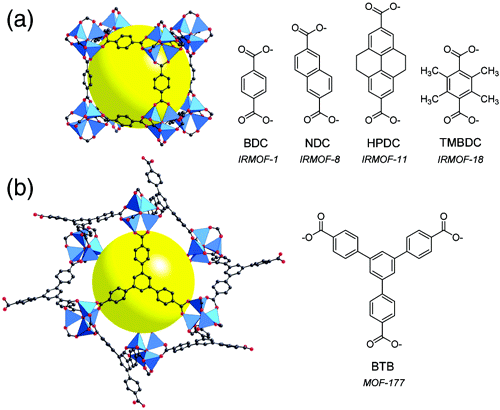
\includegraphics[width=0.55\textwidth]{figures/cited/mof-different-linker}
    \caption{Examples of two MOFs built with a zinc oxide cluster with the same
    coordination geometry. (a) Structure of MOF-5, made with a linear linker.
    (b) Structure of MOF-177, made with a trigonal linker. Image from
    reference~\cite{Rowsell2004}.}
    \label{fig:mof-different-linkers}
\end{figure}

\subsubsection{High diversity of structures}

One of the main advantage of MOFs over other porous materials such as zeolites
or activated carbons is the diversity of structures that can be built from the
different available inorganic clusters and organic linkers (see
figure~\ref{fig:mof-building-blocks}). With all the diversity provided by the
coordination and organic chemistry, one is only limited by the thermodynamic
stability of the structures obtained, and by the existence of a synthetic route
to generate the porous polymorph of interest, when another phase might be more
stable. This diversity of structure gave rise to a \emph{design to applications}
approach, where one aims at producing the best structure for a given
functionality. For example, researchers have reported MOFs with the highest
methane\cite{Tian2017} or hydrogen\cite{Oh2017} uptakes until now.

\begin{figure}[hb]
    \centering
    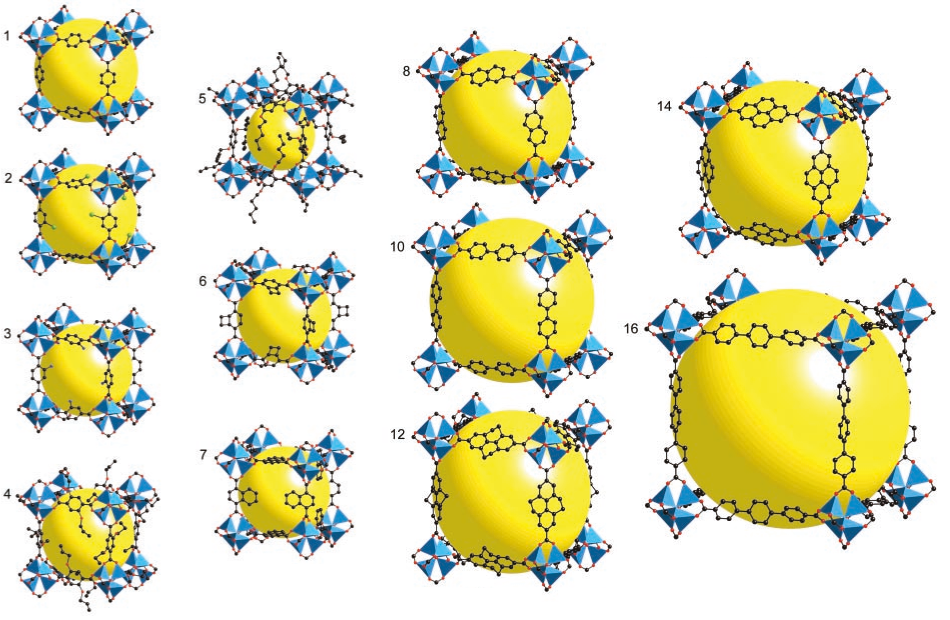
\includegraphics[width=0.75\textwidth]{figures/cited/irmof-all-sizes}
    \caption{Structures of the IRMOFs-n (n = 1-8, 10, 12, 14, and 16). Zinc
    metallic polyhedra are in blue, carbon atoms in black, oxygen in red. The
    yellow sphere represent the porous volume of each structure. Image from
    reference~\cite{Eddaoudi2002}.}
    \label{fig:irmof-all-sizes}
\end{figure}

\begin{figure}[htp]
    \centering
    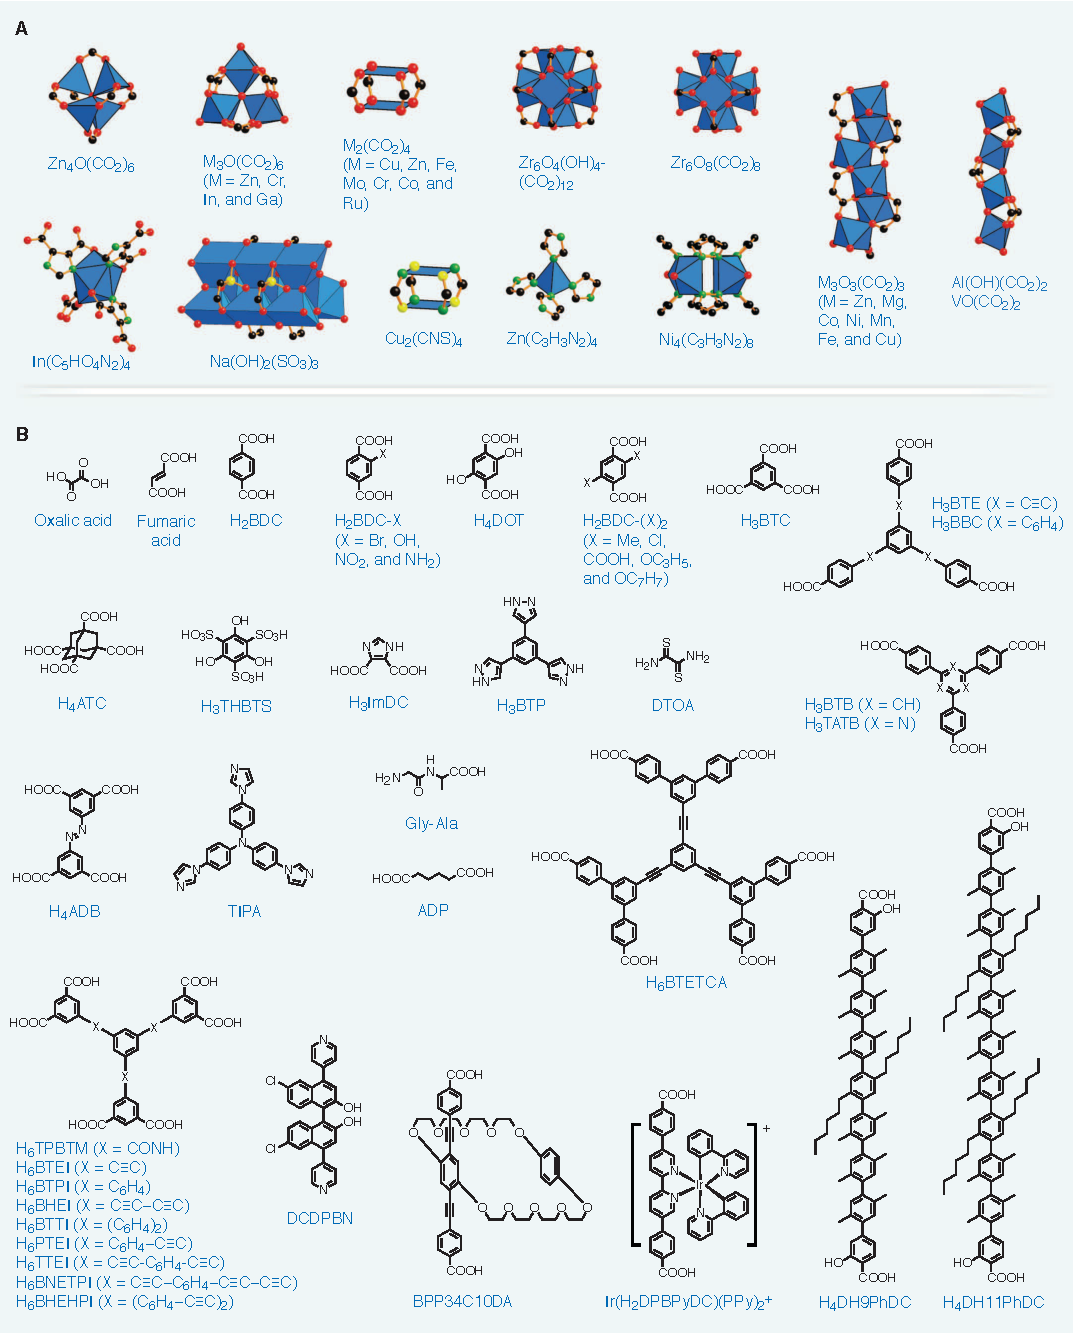
\includegraphics[width=\textwidth]{figures/cited/mof-building-blocks}
    \caption{Examples of inorganic clusters (A) and organic linkers (B) used in
    MOF synthesis. Image from reference~\cite{Furukawa2013}.}
    \label{fig:mof-building-blocks}
\end{figure}

They are two approaches used to create new MOF structures. The first one is to
use linkers and metallic centers with different connectivity, such as the ones
showed in figure~\ref{fig:mof-different-linkers}. Most of the linkers used in
MOF present either carboxylate or nitrogen organic functions that bind the
metals. Using a linker with a different number of these functions or a metal
center with different oxidation degree will create a new structure. The second
way to create a new structure is by changing the linker chemistry, while keeping
the number and positions of binding functions intact. The resulting structures
are said to be \emph{isoreticular}, \ie they share the same topology or net.

\newpage
\subsection{Zeolitic Imidazolate Frameworks}

\begin{figure}[ht]
    \centering
    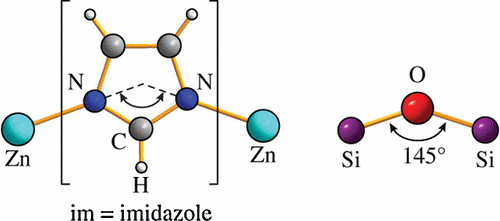
\includegraphics[width=0.4\textwidth]{figures/cited/zeolite-to-zif}
    \caption{Illustration of the analogy between ZIFs and zeolite coordination.
    Image taken from reference~\cite{Bennett2010}}
    \label{fig:zeolite-to-zif}
\end{figure}

\emph{Zeolitic Imidazolate Framework} or ZIFs is a family of MOFs built around
tetravalent metal centers such as Fe, Co, Zn, Cd or Cu; linked together by
imidazolate linkers. They present the same topology as zeolites, with
metal(imidazolate)$_2$ building blocks taking the role of \ce{SiO2} --- as
illustrated in figure~\ref{fig:zeolite-to-zif}. The first ZIFs (ZIF-1 to ZIF-12)
were synthesized in 2006\cite{Park2006}, and found to be more resistant to water
and heat that typical MOFs, which made them interesting for commercial
applications.

\begin{figure}[ht]
    \centering
    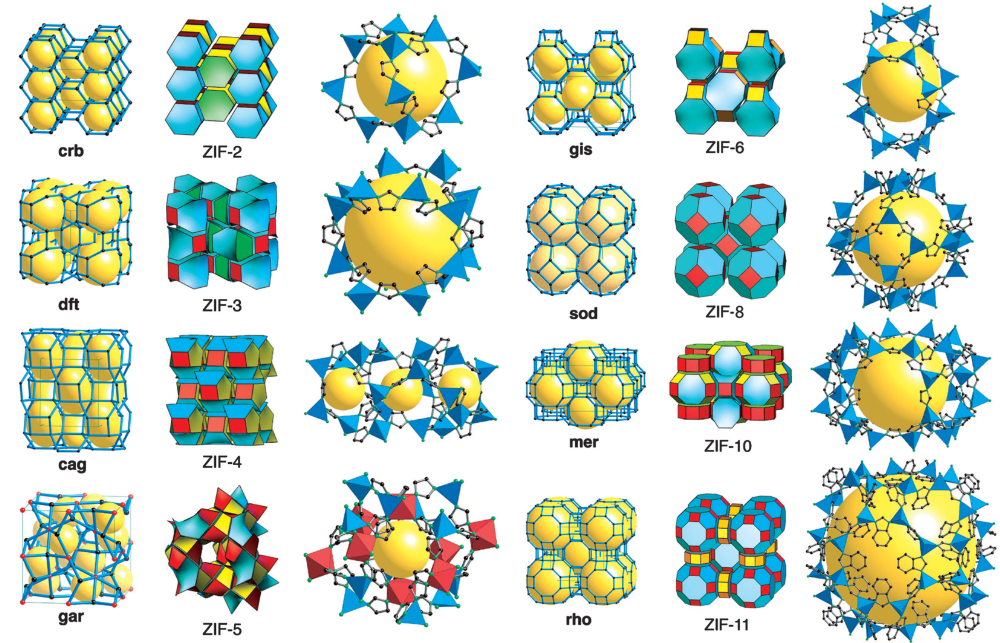
\includegraphics[width=\textwidth]{figures/cited/zif-examples}
    \caption{Examples of ZIF structures. From left to right are the crystalline
    structure of a zeolite with the same topology, the crystalline structure of
    the ZIF and the biggest sphere inside the cages. Image taken from
    reference~\cite{Park2006}}
    \label{fig:zif-examples}
\end{figure}

\ZIF8 is the member of the ZIF family which I worked on specifically during my
PhD. It uses 2-methylimidazolate (mim) as a linker, and \ce{Zn^2+} as its
metallic centers. \ZIF8 has formula \ce{Zn(mim)2} and adopts the sodalite
(\textbf{sod}) topology. In this topology, large quasi-spherical pores
corresponding to the sodalite cages are connected by windows formed by 6 and 4
zinc atoms. In \ZIF8, the 4 members windows are too small for any molecules to
go through, and all of the connectivity of the pore space happens though the 6
members windows.

\subsection{Structural flexibility}

In 1998, Susumu Kitagawa proposed a classification of MOFs in three
categories\cite{Horike2009}, depending on their behavior with respect to
molecule adsorption and desorption. The first category of materials have a
non-permanent porosity in the sense that if we remove the solvent molecules from
the structure after the synthesis the material collapses. The second category
regroups materials that have a strong enough crystalline structure and keep the
same porosity during adsorption and desorption. They are essentially rigid, and
generally present a very good mechanical and thermal stability. The last
category contains materials that retain porosity when the synthesis solvent is
removed, but may deform and change shape during adsorption.  Materials in this
last category are called \emph{Soft Porous Crystal}, and have a flexible,
dynamic structure that can change under external stimuli such as mechanical
pressure, adsorption, temperature, or even light\cite{Kitagawa2005,
Coudert2015}.

\begin{figure}[ht]
    \centering
    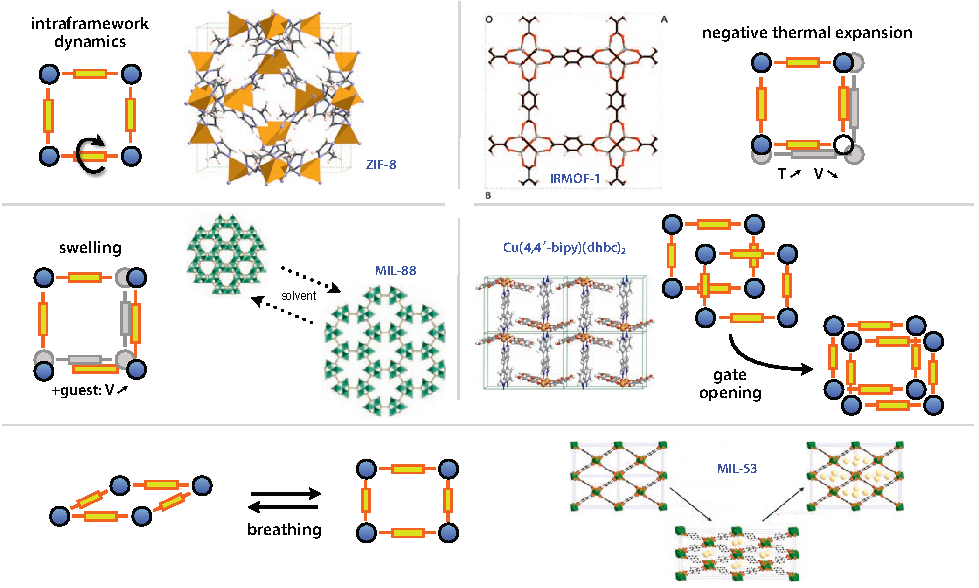
\includegraphics[width=\textwidth]{figures/cited/mof-flexibility}
    \caption{Illustration of the main flexibility modes of MOFs: linkers
    rotation, thermal expansion, swelling, gate opening and breathing. Image
    taken from reference~\cite{Coudert2011}.}
    \label{fig:mof-flexibility}
\end{figure}

This flexibility is inherent to the hybrid organic-inorganic nature of MOFs.
Indeed, their structure is based on both strong covalent bonds inside the
organic linkers, and weaker bonds such as coordination bonds, $\pi$-stacking of
linkers, hydrogen bonds, \etc These weaker bonds can vary locally in length or
orientation, inducing large scale deformations of the materials. Possible
deformation modes for MOFs are represented in figure~\ref{fig:mof-flexibility}.
All MOFs are flexible through local deformations, such as linkers rotation. This
type of flexibility happens without any global framework deformations. For other
materials we observe a volume contraction as they heat up, this phenomenon is
called \emph{negative thermal expansion}\cite{Dubbeldam2007}.

In soft porous crystal, we also observe large scale deformations of the
structure. For some materials, the whole structure will swell in presence of a
solvent. For example, the volume of MOFs of the MIL-88 family can grow to 207~\%
of the initial volume in presence of lutidine\cite{Serre2007}. Some MOFs present
multiple stable phases, and can switch from one phase to another under external
stimuli. The \emph{gate opening} phenomenon is one of such transitions, between
an initially non-porous structure to a more open and more porous structure
through the movement of linkers or the displacement of a sub-network. Materials
from the MIL-53 family also present two transitions, from an open to a
close-pore phase, and then back to an open-pore phase\cite{Serre2002} under
continuous gas loading increase.

\subsection{Industrial applications}

Zeolites enjoy a wide range of applications, from air separation using pressure
swing adsorption\cite{Rege1997}, catalysis in oil refining\cite{Primo2014},
waste water cleaning and heavy metal removal\cite{Curkovi1997}, capture of
radioactive particles\cite{Borai2009}, molecular sieve\cite{Flanigen1978}, and
even laundry detergent\cite{Karge1989}. Each year, almost 3 million tonnes of
zeolites are produced or extracted to satisfy the demand. MOFs are still
relatively new, and don't enjoy as many commercial and industrial applications
as zeolites yet. One of the obstacles to a wider usage of MOFs is their price,
as they can be a hundred times more expensive than zeolites. In the following, I
will give examples of potential applications of MOFs in various fields.

\subsubsection{Gas separation, purification and storage}

Gas separation and purification processes are at the root of the chemical
industry, either generating small carbon chains molecules from oil and natural
gas, separating oxygen from nitrogen in the air, or \ce{CO2} from \ce{H2} during
ammonia production. Current best estimates indicate that gas separation account
for 10-15~\% of the energy consumed globally. Furthermore, when faced with
climate change resulting from continually-increasing anthropogenic \ce{CO2}
emissions, optimization of storage and separation processes is increasingly
critical. They are nowadays multiple techniques used for gas separation using
cryogenic separation, liquid phase adsorption or gas phase adsorption.

As porous materials with huge specific surface area, MOFs seems like ideal
candidates for any application involving gas adsorption. Separating gases by
adsorption requires different interactions between the porous material and the
different adsorbates. These interactions can be tuned in MOFs by changing the
linkers and modifying the pores size, shape and chemical properties. During gas
purification, one chemical specie is present in majority (the gas to purify) and
we try to remove the remaining impurities. For example, HKUST-1 (a MOF with
formula \ce{Cu3(btc)2}) turned out to be very efficient to remove sulfur
compounds such as tetrahydrothiphene and thiophene from natural gas, thanks to
the formation of a \ce{Cu-S} bond\cite{Mueller2006}. It was able to adsorb
\SI{70}{g} of tetrahydrothiphene by liter of material, which is noticeably
better than the standard materials used in the industry (less than \SI{10}{g/L}
for activated carbons).

Considering gas storage, an emerging application is the storage of hydrogen gas
for energy generation and automobile transportation. Historically, hydrogen has
been stored through liquefaction or compression in bottles and tanks, but these
approaches have security and cost issues. MOFs are interesting as safer media
for gas storage because they are able to pack the hydrogen molecules densely at
a lower pressure. For example, \ce{Ni2(\textit{m}-dobdc)} is one of the current
best candidate for \ce{H2} storage, able to adsorb \SI{11}{g/L} of \ce{H2} at
ambient temperature, and up to \SI{23}{g/L} via a temperature swing from -75°C
to 25°C\cite{Kapelewski2018}.

\subsubsection{Heterogeneous catalysis}

Heterogeneous catalysis is used in numerous industrial processes. Selectivity of
these catalytic processes is often based on the shape and size of the reactants,
hence the interest in using catalysts with a regular and uniform porosity.
Porous crystalline materials are especially interesting in this regard.
Moreover, since catalysts can be re-used, and only small quantities of them are
needed, the advantages of MOFs can offset their cost. The possibilities to
create chiral MOFs using enantiomerically pure linkers, or conformational
chirality\cite{Tshabang2018} also opens the way to asymetric catalysis.

A first strategy for using MOFs as catalysts involves the metallic centers,
which can have a catalytic activity of their own. For example, MIL-100(Fe) and
MIL-100(Cr) have an interesting activity for the Friedel-Craft benzylation
reaction, used for the production of linear alkyl-benzene; surpassing the
activity of the HBEA and HY zeolites traditionally used\cite{Horcajada2007}.
HKUST-1 MOF can be activated after the synthesis by removing an apical water
molecule, creating a very reactive Lewis acid site which can be used for
cyanosilylation reactions\cite{Schlichte2004}.

Another approach for adding catalytic activity to MOFs entails adding functional
groups to the linkers with the desired activity. For example, SALEM-2 can be
activated with \mbox{n-butyllithium} and exhibits a strong Brønsted base
catalytic activity\cite{Karagiaridi2012} (see figure~\ref{fig:zif8-to-salem2}).
Around the same idea, the amino functions of IRMOF-3 and amino-MIL-53 makes them
suitable as basic catalysts for the Knoevenagel condensation of
ethyl-cyanoacetate and ethyl-acetoacetate with benzaldehyde\cite{Gascon2009}.

\begin{figure}[ht]
    \centering
    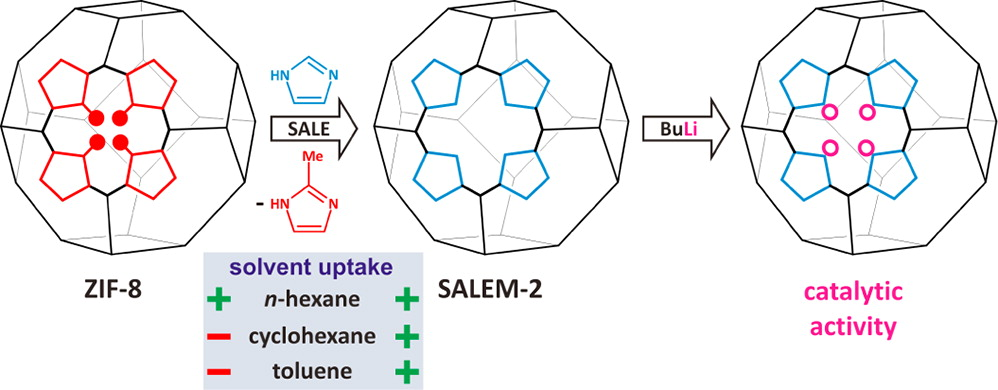
\includegraphics[width=0.65\textwidth]{figures/cited/zif8-to-salem2}
    \caption{Post-synthetic modifications of \ZIF8 to synthesize SALEM-2 and
    obtain catalytic activity. Image taken from reference~\cite{Karagiaridi2012}.}
    \label{fig:zif8-to-salem2}
\end{figure}

\subsubsection{Chemical sensors}

Some MOFs have luminescent properties, linked either to the presence of aromatic
or functionalized linkers or a metal cation from the lanthanide group. These
luminescent properties, combined with the adsorption capabilities of MOFs open
the possibility of using MOFs as chemical sensors. The structural and/or
electronic transition of a MOF upon adsorption will modify the light emission
properties of the material, allowing to detect specific gaseous compounds. This
is particularly interesting to detect explosive materials. For example, the
\ce{Zn2(bpdc)2(bpee)} MOF is able to detect multiple nitro- substituted
molecules found in explosives such as 2,4-dinitrotoluene or
2,3-dimethyl-2,3-dinitrobutane in around \SI{10}{s}\cite{Lan2009} (see
figure~\ref{fig:chemical-sensor}). Another example is the \ce{[Zn2(oba)2(bpy)]3}
MOF, also able to detect explosive and aromatic molecules through a fluorescence
quenching phenomenon\cite{Pramanik2011}.

\begin{figure}[ht]
    \centering
    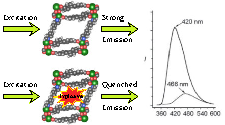
\includegraphics[width=0.55\textwidth]{figures/cited/chemical-sensor}
    \caption{Schematic representation of optical properties modifications of
    \ce{Zn2(bpdc)2(bpee)} MOF. Image adapted from reference~\cite{Lan2009}.}
    \label{fig:chemical-sensor}
\end{figure}

\section{Adsorption and intrusion}

Adsorption is a surface phenomenon, where molecules or atoms are creating a film
at the surface of a material. Because they have a high specific surface area,
the adsorption in porous materials is higher than on bulk materials. Adsorption
is used as a characterization technique for such porous media, and is also the
basis for their most prevalent applications.

\subsection{Studying adsorption}

It is possible to study adsorption both with experimental and theoretical
approaches. The central tool for the study of adsorption is the single component
adsorption isotherm. Considering a pure gas adsorbing in a porous matrix, the
isotherm adsorption records the amount of adsorbed gas at a fixed temperature as
a function of the pressure, or the more commonly, the pressure relative to the
vapor pressure of the gas. Experimentally, these adsorption isotherms are
obtained with gravimetric, volumetric or chromatographic
methods\cite{Ruthven1984, Yang1987}.

\begin{figure}[htb]
    \centering
    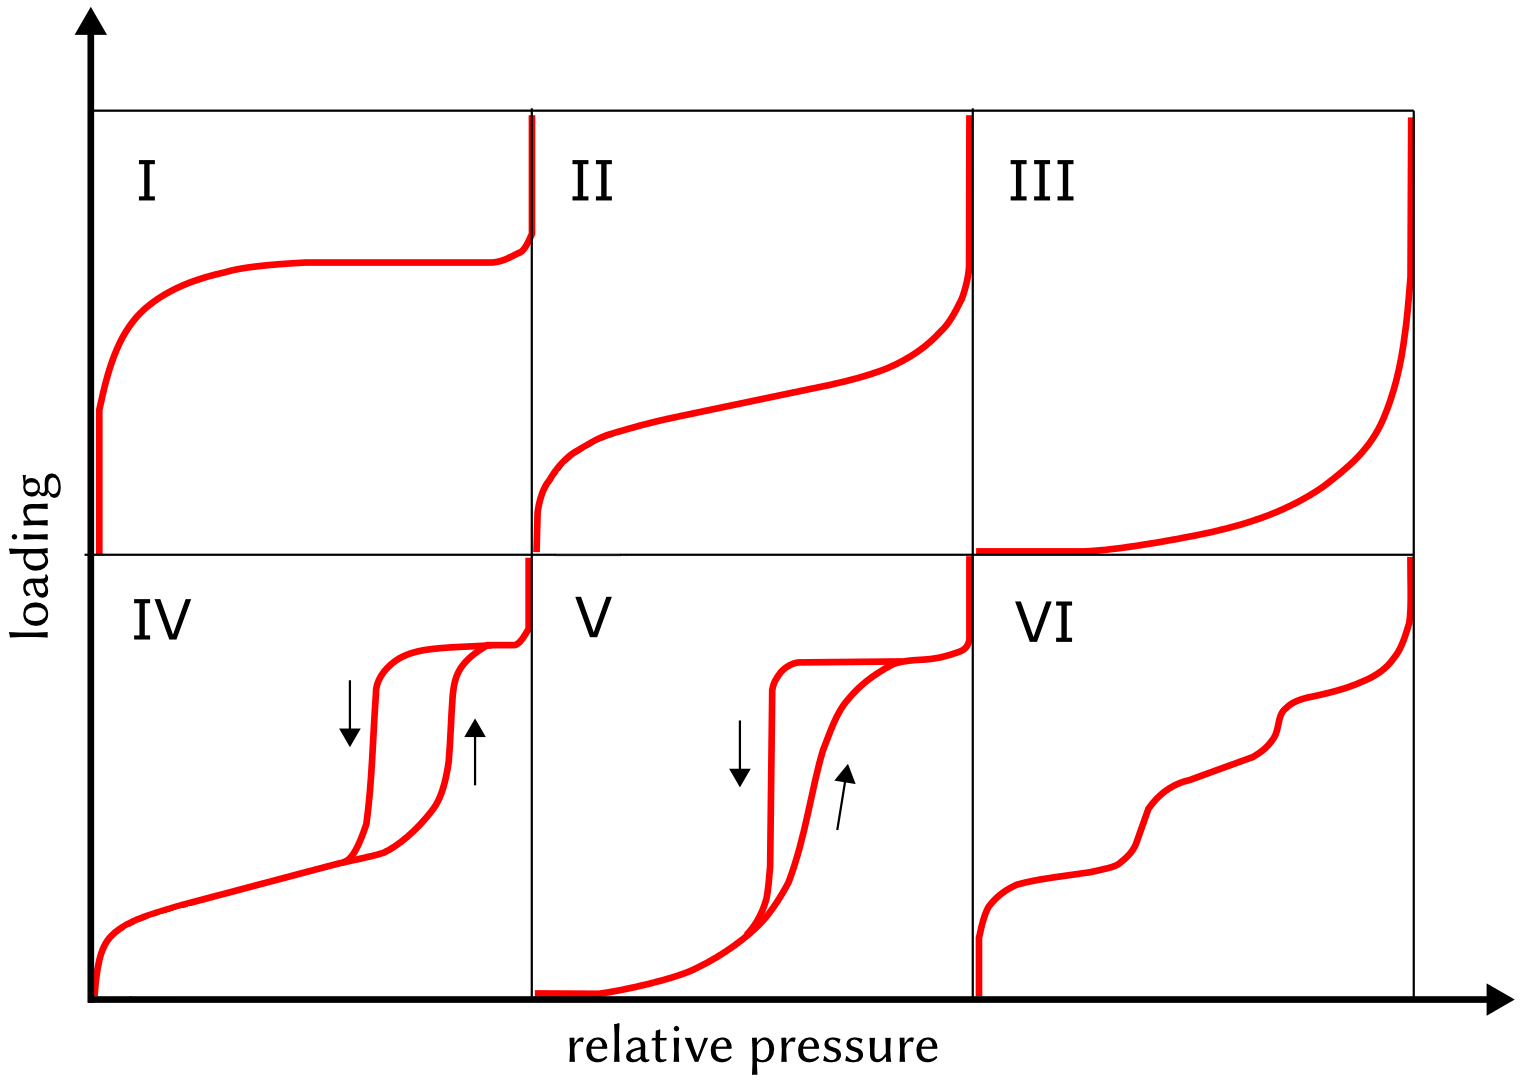
\includegraphics[width=0.75\textwidth]{figures/images/iupac-isotherms}
    \caption{IUPAC classification of isotherms.}
    \label{fig:iupac-isotherms}
\end{figure}

The IUPAC classify adsorption isotherms depending on their shape, as represented
in figure~\ref{fig:iupac-isotherms}\cite{Sing1985}. Only the isotherms of type
I, IV and V can occur in nanoporous solids. Type I isotherms are concave,
reversible and the adsorbed quantity of matter (or \emph{loading}) goes to a
finite value as the pressure increases. It is the most common isotherm type, and
express the prevalence of gas--solid interactions over gas--gas interactions in
a material containing a single kind of equivalent adsorption sites. Type IV
isotherms also present a maximal loading, and one or two steps with sometimes an
hysteresis loop between the adsorption and desorption branches. These steps are
usually attributed to a modification in the structure of the adsorbing
solid\cite{Karge1989}. Type V isotherm shows an inflection point: at low pressure
the adsorption is very low, mainly due to small gas--solid interactions. For
higher pressures the adsorption becomes stronger thanks to interactions between
the gas molecule themselves. In flexible porous materials, type IV isotherms
would be associated with \emph{breathing} materials, and type V isotherms with
\emph{gate opening}. Finally, isotherms types II, III and VI do not present a
maximal loading, and are usually observed in solids with multiple pore sizes and
a continuous transition from mono-layer adsorption to multi-layers adsorption and
capillary condensation.

Is is possible to study and predict adsorption isotherms by using thermodynamics
and molecular simulations methods such as Grand Canonical Monte Carlo. I will
present with more details the theoretical methods I used during my PhD to study
adsorption in the corresponding chapters: chapter~\ref{sec:macrosopic} for
macrosopic thermodynamics modelling; and chapter~\ref{sec:molsim} for molecular
simulations.

\subsection{Intrusion: high pressure adsorption}


\subsubsection{Intrusion of water in hydrophobic materials}

Nanoporous crystalline materials such as zeolites, metal--organic frameworks
(MOF), carbon nanotubes and inorganic open frameworks enjoy a wide range of
applications, ranging from catalysis, fluid separation and purification, to gas
capture and detection of dangerous molecules. The fundamental basis for most of
these applications is the material's capability to adsorb large quantities of
molecules inside its nanometer-sized pores, due to its large specific surface
area. In this context, hydrophobic nanoporous materials offer the advantage that
the uptake of water from the gas phase --- e.g., humidity in the air --- is very
small\cite{Wu2010, Ghosh2014, Wang2016}. Given that water is often strongly
adsorbed and competes with other molecules for adsorption sites, hydrophobic
molecular sieves can offer higher separation properties\cite{Flanigen1978,
Giaya2000}.

\subsection{Coupling adsorption and deformations}


\OnlyInSubfile{\printbibliography}

\end{document}
